% Author: Ben Champion <bwc3252@rit.edu>
% Main LaTeX file for Lenfest Community Weekend 2019 Presentation

\documentclass{beamer}

\usetheme{Amsterdam}

\usepackage{caption}

\begin{document}
\title{Astrophysical Parameter Inference with Gravitational Wave and Electromagnetic Data Channels}
\author{Ben Champion}
\institute{Rochester Institute of Technology \\ Center for Computational Relativity and Gravitation}

% logos
\titlegraphic{
\includegraphics[width=6cm]{Images/RIT_RGB_hor_k}\hspace*{2cm}~%
   
\includegraphics[width=2cm]{Images/ccrg_logo}
}

\date{
  \today
}

\frame{
  \titlepage
}

\frame{ \frametitle{Table of contents}
  \tableofcontents
}


\section{Introduction}

\frame{ \frametitle{Background - Special Relativity}
  \begin{columns}[c]
    \column{3.0in}
    \begin{itemize}
      \item 1905 - Einstein's theory of Special Relativity \pause
      \begin{itemize}
        \item The speed of light is independent of the motion of the observer \pause
        \item Consequences include length contraction, time dilation, etc. \pause
        \item Shortcoming: only applies to inertial (non-accelerating) reference frames \pause
      \end{itemize}
    \end{itemize}
    \column{1.5in}
    \begin{figure}
      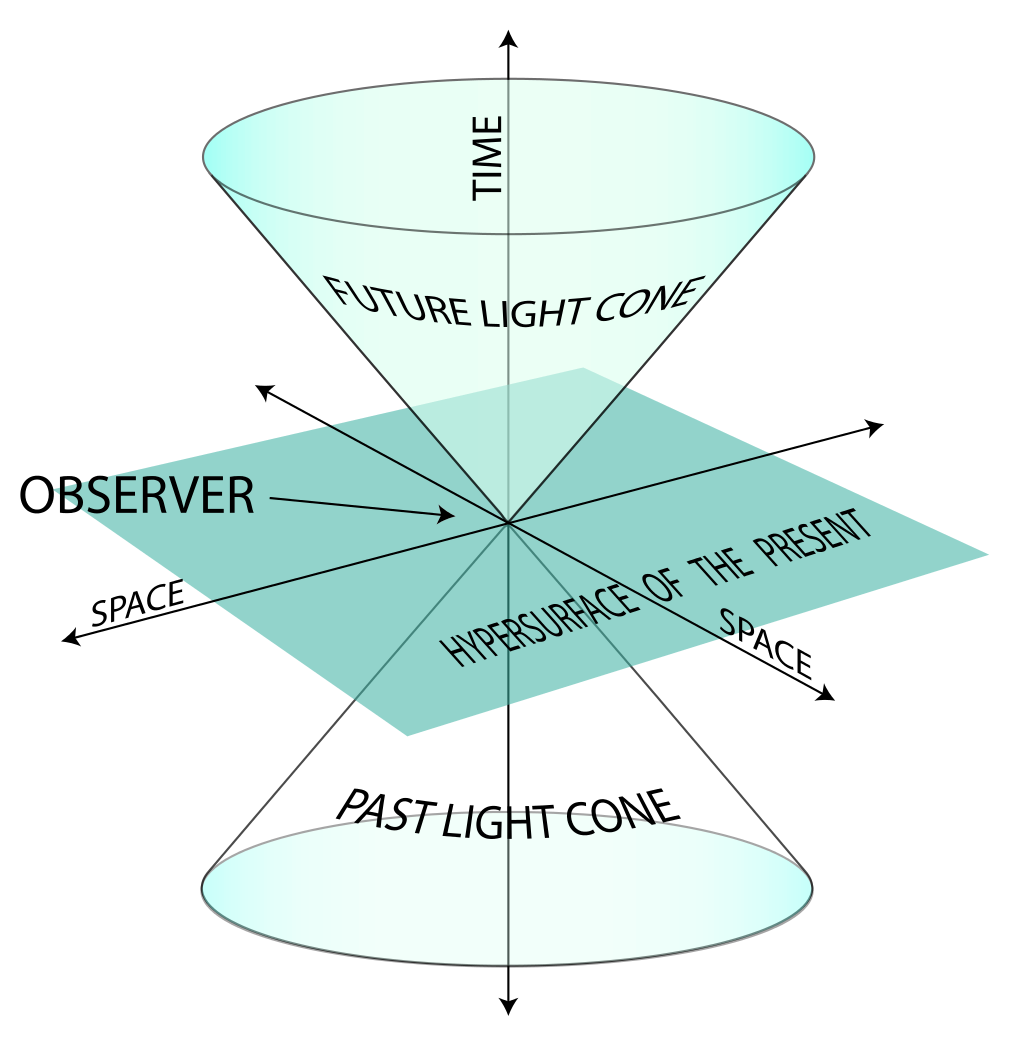
\includegraphics[width=\linewidth]{Images/world_line}
      \caption*{\fontsize{8pt}{10pt}\selectfont Lightcone: the path through spacetime that a single "flash" of light, traveling in all directions, would take (image by K. Aainsqatsi)}
    \end{figure}
  \end{columns}
}

\frame{ \frametitle{Background - Special Relativity}
  Classically, for an event with coordinates $(t, x)$ as measured by a stationary observer and $(t', x')$ as measured by an observer moving with velocity $v$:

  \begin{align*}
    t' &= t  \\
    x' &= x - vt
  \end{align*}

  \pause

  However, according to Special Relativity:

  \begin{align*}
    t' &= \gamma (t - \frac {vx} {c^2}) \\
    x' &= \gamma (x - vt) \\
    \text{where } \gamma &= \frac {1} {\sqrt{1 - \frac {v^2} {c^2}}}
  \end{align*}

  }

\section{Gravitational Wave PE}

\frame{
}

\section{Neutron Star Mergers and Kilonovae}

\frame{
}

\section{Joint GW/EM PE}

\frame{
}

\section{Results}

\frame{
}

\end{document}
